\section{ReTex}

Retex es una propuesta de implementación de un sistema de recuperación de información textual. Retex está dividido en dos aplicaciones: 

\begin{enumerate}
    \item \textbf{Motor de búsqueda} implementado en Python utilizando una API (abreviatura de Application Programming Interface). Todo el procesamiento del motor de búsqueda se implementó en un módulo de Python cuyo nombre es \verb|retex|, y la API se implementó utilizando la librería de Python \verb|FastAPI|.
    \item \textbf{Interfaz visual} implementado en VueJS, framework para el desarrollo de frontend en aplicaciones webs.
\end{enumerate}

\subsection{Motor de búsqueda}

El motor de búsqueda se basa en el modelo vectorial de recuperación de información, el cual se define como sigue. Un Modelo Vectorial de Recuperación de Información \cite{manning} no es más que una tupla $<D, Q, F, R>$ donde:

\begin{enumerate}
    \item[$\bullet$] $D$: Vectores de los pesos asociados a los términos  de los documentos. Estos pesos $w$ son no binarios y mayores que cero ($w > 0$)
    \item[$\bullet$] $Q$: Vector de los pesos asociados a los términos de la consulta.
    \item[$\bullet$] $F$: Espacio $n$ dimensional y operaciones entre vectores del álgebra lineal
    \item[$\bullet$] $R$: Función de ranking, generalmente es el coseno entre el vector de pesos de la consulta y los vectores de los documentos.
\end{enumerate}

El motor de búsqueda implementado sigue el flujo mostrado en la Fig \ref{esq}, donde el usuario realiza una consulta $q$ en forma de texto a través de la interfaz visual. La consulta $q$ se convierte en una instancia de la clase \verb|Query|, donde se almacenan las palabras claves de la misma, y se almacenan los pesos de cada término. Esta consulta se introduce en el modelo vectorial, pero antes de esto se revisa en la caché de consultas, si $q$ está se devuelven los resultados de la misma, si $q$ no está entonces se introduce en el modelo y se calcula el ranking $R$ de los documentos relevantes a $q$, donde el documento $R_1$  es el más relevante y por lo tanto tiene mayor similitud con la consulta $q$ del usuario.

\begin{figure}\label{esq}
    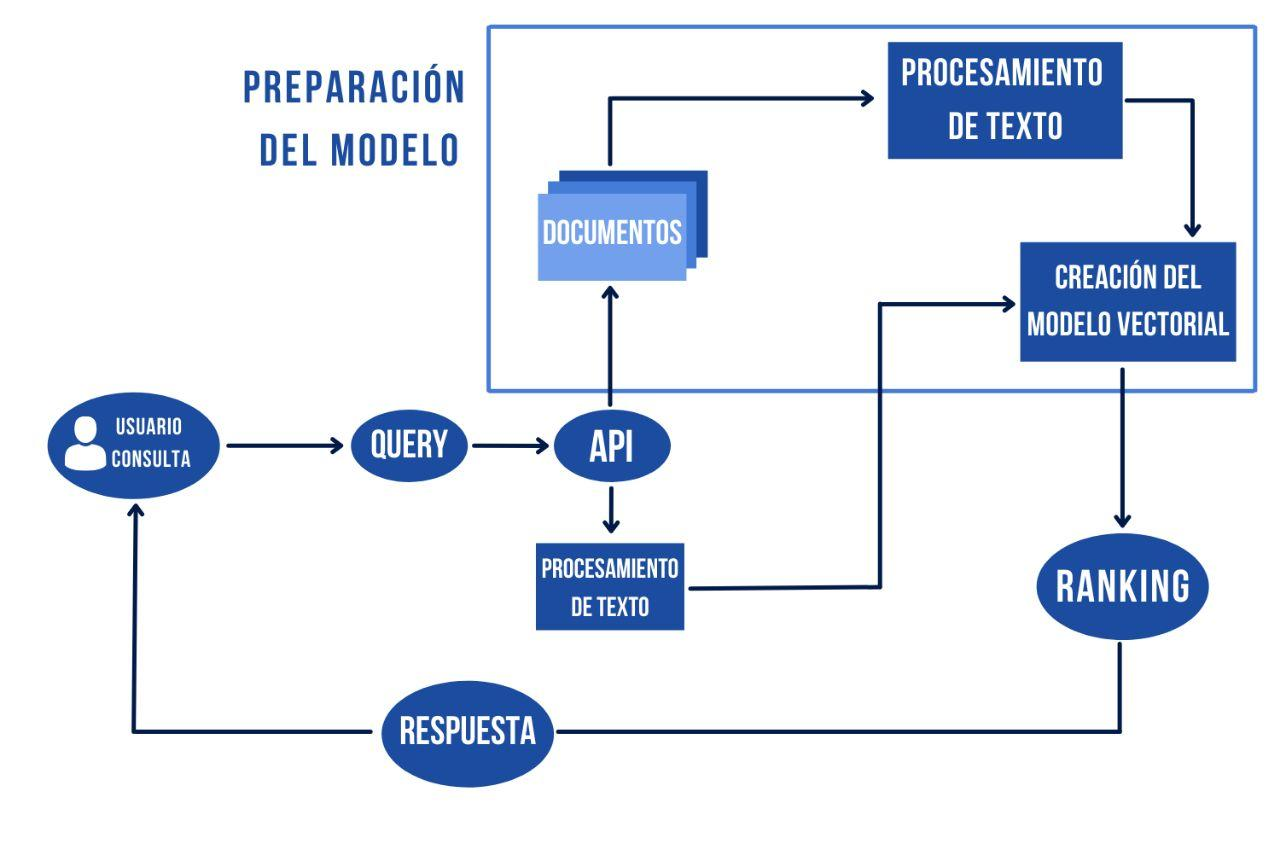
\includegraphics[width=10cm]{sections/img/esq.jpg}

    \caption{Flujo del motor de búsqueda}
\end{figure}

La preparación del modelo consiste en lo siguiente: se cargan todos los documentos de la colección utilizando una clase que herede de \verb|Parser| según convenga para la colección. Las clases concretas de la clase abstracta mencionada separan todos los docuementos y sus metadatos en instancias de la clase \verb|BaseDocument| o clases concretas de \verb|BaseDocument| según convenga para la colección.

Luego de tener una lista con todos los documentos de la colección se procede a procesar los textos de los documentos y posteriormente extraer las palabras claves o los términos de los documentos. 

En el procesamiento de texto se utilizó la librería de Python \verb|nltk| y se realizaron los siguientes procedimientos:

\begin{enumerate}
    \item Eliminación de los signos de puntuación.
    \item Eliminación de stopwords: palabras que no aportan información alguna al modelo, ni permiten decidir en qué categoría se debe clasificar el texto. Por ejemplo: preposiciones, conjunciones, entre otras.
    \item Normalización de los documentos a minúscula. 
    \item Aplicación de la lemantización.  La lemantización es un proceso lingüístico que consisten en dada una forma flexionada hallar el lema correspondiente. Por ejemplo: el lema de la palabra jóvenes es joven. Es decir, el lema de una palabra es aquella que se encuentra como entrada de un diccionario tradicional, esto es singular para los sustantivos, masculino singular para adjetivos, y el infinitivo para los verbos.
\end{enumerate}

Para la extracción de palabras claves se implementó una clase \verb|Indexer| que dado una colección de docuementos devuelve para cada uno los términos y sus pesos asociados. Se exploraron dos enfoques principales en la selección de palabras claves o términos:

\begin{enumerate}
    \item[$\bullet$] \verb|NaiveIndexer|, en el cual todas las palabras del documento son palabras claves.
    \item[$\bullet$] \verb|NounIndexer|, en el cual solo los sustantivos presentes en los documentos son palabras claves. En el artículo Relevance Weighting of Search Term \cite{re} se plantea que los sustantivos de un documento tienden a expresar la temática del mismo. 
\end{enumerate}

Luego de experimentar con ambos enfoques se decidió adoptar el \verb|NounIndexer| como mecanismo de selección de palabras claves para el motor de búsqueda. Posterior a todo este procesamiento se tiene un lista de vectores $K$ de palabras claves.

\begin{verbatim}
class Indexer(ABC):
  def __call__(self, docs_text: List[str]):
      vocabulary = self.extract_vocabulary(docs_text)
      vectorize = TfidfVectorizer(vocabulary=vocabulary)
      weight = vectorize.fit_transform(docs_text)
      idf = vectorize.idf_
      tf = [w / idf for w in weight]
      return (weight, idf, tf, vectorize.get_feature_names_out())
  @abstractmethod
  def extract_vocabulary(self, docs_text: List[str]) -> List[str]:
    pass

class NounIndexer(Indexer):
  def extract_vocabulary(self, docs_text: List[str]) -> List[str]:
    is_noun = lambda pos: pos[:2] == 'NN'
    stop_words = set(stopwords.words('english'))
    nouns: Set[str] = set()
    for doc in docs_text:
        tokenized = word_tokenize(doc)
        tokenized = [WordNetLemmatizer().lemmatize(w) for w in tokenized]
        tokenized = [token for token in tokenized if not token in stop_words]
        for (word, pos) in pos_tag(tokenized):
            if is_noun(pos):
                nouns.add(word)
    return list(nouns)
\end{verbatim}

\subsubsection{Ponderación de términos en el motor de búsqueda}

Luego de tener los términos de cada documento es necesario obtener los pesos asociados a cada uno de estos términos. Para ello se utilizó la clase \verb|TfIdfVectorizer| \cite{tf} \cite{tfidf} de la librería \verb|sklearn| de Python, que tiene el siguiente funcionamiento implementado de forma eficiente:

Se calcula la frecuencia $f_i$ de aparición de cada término en los documentos y se calcula el $tf_{ij}$ que corresponde a la frecuencia normalizada del término $i$ en el docuemnto $j$ de la colección. La expresión de $tf_{ij}$ es la siguiente:

$$ tf_{ij} = \frac{f_i}{max_l f_l} $$

Y luego se calcula el $idf_i$ para cada término, que representa la frecuencia de ocurrencia del término $i$ dentro de todo los documentos, dada por la siguiente ecuación:

$$ idf_i = \log \bigg(\frac{N}{n + 1}\bigg) $$

donde $N$ representa la cantidad de documentos en el sistema y $n$ la cantidad de documentos en los que aparece el término $i$, se modificó la expresión sumando 1 en el denominador del argumento del logaritmo para evitar errores por las divisiones por 0, en caso de que el término no se encuentre en ningún documento.

Posteriormente el peso del término $i$ en el documento $j$ se define como:

$$ tfidf_{if} = w_{ij} = idf_i * tf_{ij} $$

Luego de esto, se tiene una lista de vectores que contienen los términos y los pesos asociados a cada término en un documento.

\subsubsection{Procesamiento de consultas}

Una consulta es una cadena de texto que expresa las necesidades de información del usuario, por tal razón se realiza el mismo procesamiento de texto que a los documentos, como la lemantización, eliminación de palabras claves y se calculan los pesos asociados a las palabras claves de la consulta.

Para el cómputo de los pesos de una consulta se introduce el valor $\alpha$ que se conoce como constante de suavizado. Este permite amortiguar la variación en los pesos de términos que ocurren poco, para evitar, por ejemplo, grandes saltos entre la frecuencia de un término que aparece una vez a otro que aparece dos veces.

Por tanto, la ecuación de los pesos de los términos de la consulta es la siguiente:

$$ w_{iq} = \bigg(\alpha + (1 -\alpha) tf_{iq}\bigg) * idf_i  $$

\subsubsection{Construcción del ranking}

Como se expresa en la definición formal del modelo vectorial se tiene una función de similitud $R$ que calcula la similitud entre la consulta y los documentos. En este caso se utilizó el coseno del ángulo formado por el vector de pesos $w_q$ de la consulta y el vector de pesos de cada documento, cuya expresión es la siguiente:

$$ sim(q, d) = \frac{\sum_{i = 1}^n w_{id} * w_{iq}}{\sqrt{\sum_{i=1}^n w_{id}^2} \sqrt{\sum_{d=1}^n w_{iq}^2}} $$

Para ello se utilizó la función \verb|cosine_similarity| \cite{cos} de la librería \verb|sklearn|, que implementa esta expresión de forma eficiente y rápida.

Luego de que se tiene calculado esta medida de similitud para cada uno de los documentos se introducen todos los elementos en un Heap, implementado en la librería \verb|heapq| de Python y se exploraron dos enfoques para la construcción del ranking.

\begin{enumerate}
    \item[$\bullet$] \textbf{Top-rank:} se tiene un parámetro \verb|top| que representa la cantidad de elementos que existirán en el ranking, o sea el ranking será un conjunto de aridad \verb|top| donde están los documentos con mayor valor de la función $sim$.
    \item[$\bullet$] \textbf{Threshold-rank:} se tiene un parámetro \verb|threshold| que representa un umbral para construir el ranking, el cual estará compuesto por todos los documentos cuyo valor de la función $sim$ se mayor que el parámetro \verb|threshold|. El ranking será un conjunto de aridad variable. 
\end{enumerate}

Luego de explorar ambos enfoques se decidió fusionarlos de la siguiente forma, se calcula el valor $sim$ para cada documento, y luego se calcula el Top-rank y se almacenan aquellos documentos cuyo valor de la función $sim$ se mayor que el umbral. 

\begin{verbatim}
def get_posting_list(self, framework, qry, wq):
    wc = framework.weigths
    cos = cosine_similarity(wc, wq.reshape(1, -1))

    doc_cos = []
    for i in range(len(framework.collection)):
        doc = framework.collection[i]
        sim = cos[i]
        doc_cos.append((doc, sim))

    umbral = Config().get_umbral()

    top = nlargest(self.top, doc_cos, key=lambda x: x[1])
    top = list(filter(lambda t: t[1] > umbral, top))
    top = list(map(lambda t: t[0], top))
    return top
\end{verbatim}

\subsection{Evaluación del motor de búsqueda}

Para la evaluación del motor de búsqueda se utilizaron 4 medidas de evaluación: la precisión, el recall, medida $F$ y la medida $F1$. Veamos que representa cada una de estas:

\begin{enumerate}
    \item[$\bullet$] \textbf{Precisión:} la fracción de documentos recuperados que son relevantes y está dada por la siguiente expresión, $P = \frac{|RR|}{|RR \cup RI|}$ donde $RR$ es el conjunto de los documentos relevantes recuperados y $RI$ es el conjunto de documentos irrelevantes recuperados.
    \item[$\bullet$] \textbf{Recall o recobrado:} la fracción de documentos relevantes que son recuperados, y está dada por la siguiente expresión $R = \frac{|RR|}{|RR \cup NR|}$ donde $NR$ representa el conjunto de documentos relevantes que no fueron recuperados.
    \item[$\bullet$] \textbf{Medida F:} permite enfatizar la precisión sobre el recall o viceversa. Está dada por la siguiente expresión $F = \frac{1 + \beta^2}{P^{-1} + \frac{\beta^2}{R}}$.
    \item[$\bullet$] \textbf{Medida F1:} permite enfatizar armonizar la precisión y recall. Es un caso particular de la medida $F$ con parámetro $\beta = 1$. 
\end{enumerate}


Se tiende a pensar que la precisión es la medida fundamental para evaluar estos sistemas dado que representa la cantidad de documentos recuperados que son relevantes, pero no siempre se quiere esto si no que se desea tener la mayor cantidad de documentos relevantes dentro de los recuperados. Por tanto, se enfatizó en mejorar el recall.

\subsection{API del motor de búsqueda}

Se implementó una API para interactuar con el motor de búsqueda, esta interfaz tiene las siguientes rutas:

\begin{enumerate}
    \item[$\bullet$] \verb|/search?q=<str>| la cual devuelve un json con todos los documentos relevantes a la consulta $q$. O sea, devuelve el ranking de documentos con mayor $sim$ para la consulta $q$.
    \item[$\bullet$] \verb|/eval| devuelve un json con los valores de las métricas de la evaluación del motor de búsqueda.
    \item[$\bullet$] \verb|/collection/:id| que devuelve un json con el documento de la colección con identificador $id$.  
\end{enumerate}

\subsection{Comportamiento del motor de búsqueda en distintos contextos}

Retex se evaluó con dos colecciones de documentos:

\begin{itemize}
    \item Cranfield \cite{cran}: colección de prueba surgida para los experimentos Cranfield, enfocados a estudiar la recuperación de información y en especial a evaluar la eficiencia de los sistemas de indexado de los años 1960. Esta colección fue desarrollada por Cyril W. Cleverdon en el Colegio de Aeronáutica, hoy conocido como la Universidad de Cranfield. La colección está compuesta por 1400 documentos en inglés, y 255 consultas, además de las relaciones de relevancia para cada consulta.
    \item Medline: colección de prueba con enfoque biomédico y ciencias naturales, incluye información bibliográfica de artículos de temas de medicina, enfermería, farmacia, estomatología, veterinaria, y salud. Esta colección fue compilada por la Biblioteca Nacional de Medicina de los Estados Unidos, lanzando su primera versión en línea en 1971. Cuenta con 1033 documentos en inglés, y 30 consultas, además de las relaciones de relevancia para cada consulta.
\end{itemize}

Se implementó una clase concreta de \verb|Parser| para cada colección así como una clase concreta de \verb|BaseDocument|. Estas clases llevan por nombre: \verb|CranParser|, \verb|MedlineParser|, y para los documentos: \verb|CranDocument| y \verb|MedlineDocument|.

A continuación se analiza el comportamiento del sistema con diferentes parámetros, por ejemplo: el umbral, el top del ranking y el valor $\alpha$. El análisis se realiza con el fin de encontrar los valores óptimos que maximicen el recobrado del sistema.

\subsubsection{Medline}

Se presenta la evaluación del comportamiento del sistema con los documentos de la colección Medline en los siguientes contextos:

\begin{itemize}
    \item Con \verb|umbral = 0.1|, \verb|top = 600| y \verb|alpha = 0.5|, el sistema tiene $P = 0.31736$, $R = 0.55088$, $F-mean = 0.33012$ y $F1 = 0.37067$.
    \item Con \verb|umbral = 0.1|, \verb|top = 600| y \verb|alpha = 0.4|, el sistema tiene $P = 0.31706$, $R = 0.54998$, $F-mean = 0.32960$ y $F1 = 0.36988$.
    \item Con \verb|umbral = 0.08|, \verb|top = 600| y \verb|alpha = 0.5|, el sistema tiene $P = 0.27365$, $R = 0.60575$, $F-mean = 0.29249$ y $F1 = 0.34415$.
    \item Con \verb|umbral = 0.08|, \verb|top = 600| y \verb|alpha = 0.4|, el sistema tiene $P = 0.27232$, $R = 0.60461$, $F-mean = 0.29107$ y $F1 = 0.34264$.
\end{itemize}

El sistema con los parámetros \verb|umbral = 0.08| y \verb|alpha = 0.5| recupera en promedio el 60.58\% de los documentos relevantes a una consulta, lo cual se puede catalogar de aceptable. 

Si se reduce el umbral tiende a mejorar el recobrado del sistema, estos son los resultados con umbral 0.05: $P = 0.19993$, $R = 0.71826$, $F-mean = 0.22077$ y $F1 = 0.27986$. 

Si se presta atención la precisión disminuye considerablemente cada vez que se disminuye el valor del umbral mientras que el recobrado aumenta considerablemente.

\subsubsection{Cranfield}

Se presenta la evaluación del comportamiento del sistema con los documentos de la colección Cranfield en los siguientes contextos:

\begin{itemize}
    \item Con \verb|umbral = 0.1|, \verb|top = 600| y \verb|alpha = 0.5|, el sistema tiene $P = 0.00875$, $R = 0.13097$, $F-mean = 0.01056$ y $F1 = 0.01545$.
    \item Con \verb|umbral = 0.1|, \verb|top = 600| y \verb|alpha = 0.4|, el sistema tiene $P = 0.00867$, $R = 0.13077$, $F-mean = 0.01047$ y $F1 = 0.01532$.
    \item Con \verb|umbral = 0.05|, \verb|top = 600| y \verb|alpha = 0.4|, el sistema tiene $P = 0.00734$, $R = 0.24694$, $F-mean = 0.00906$ y $F1 = 0.01394$.
    \item Con \verb|umbral = 0.05|, \verb|top = 600| y \verb|alpha = 0.5|, el sistema tiene $P = 0.00734$, $R = 0.24390$, $F-mean = 0.00905$ y $F1 = 0.01393$.
\end{itemize}

El sistema con los parámetros \verb|umbral = 0.05| y \verb|alpha = 0.4| recupera en promedio el 24.65\% de los documentos relevantes a una consulta, lo cual se puede catalogar de malo. 

Si se reduce el umbral tiende a mejorar el recobrado del sistema, estos son los resultados con umbral 0.005: $P = 0.00643$, $R = 0.33233$, $F-mean = 0.00797$ y $F1 = 0.01247$. 

Si se presta atención la precisión disminuye cada vez que se disminuye el valor del umbral mientras que el recobrado aumenta pero no se llegan a resultados aceptables.

\subsection{Interfaz visual de Retex}

La interfaz visual de Retex siguió la línea de diseño de Google, y fue implementado utilizando VueJS y Bootstrap. Su página principal tiene un formulario para realizar las consultas y redirecciona a una página donde se muestra el ranking y se puede acceder a los documentos relevantes a la consulta. Además se muestra la evaluación del sistema.

A continuación se muestran algunas imágenes de la interfaz visual:

\begin{figure}
    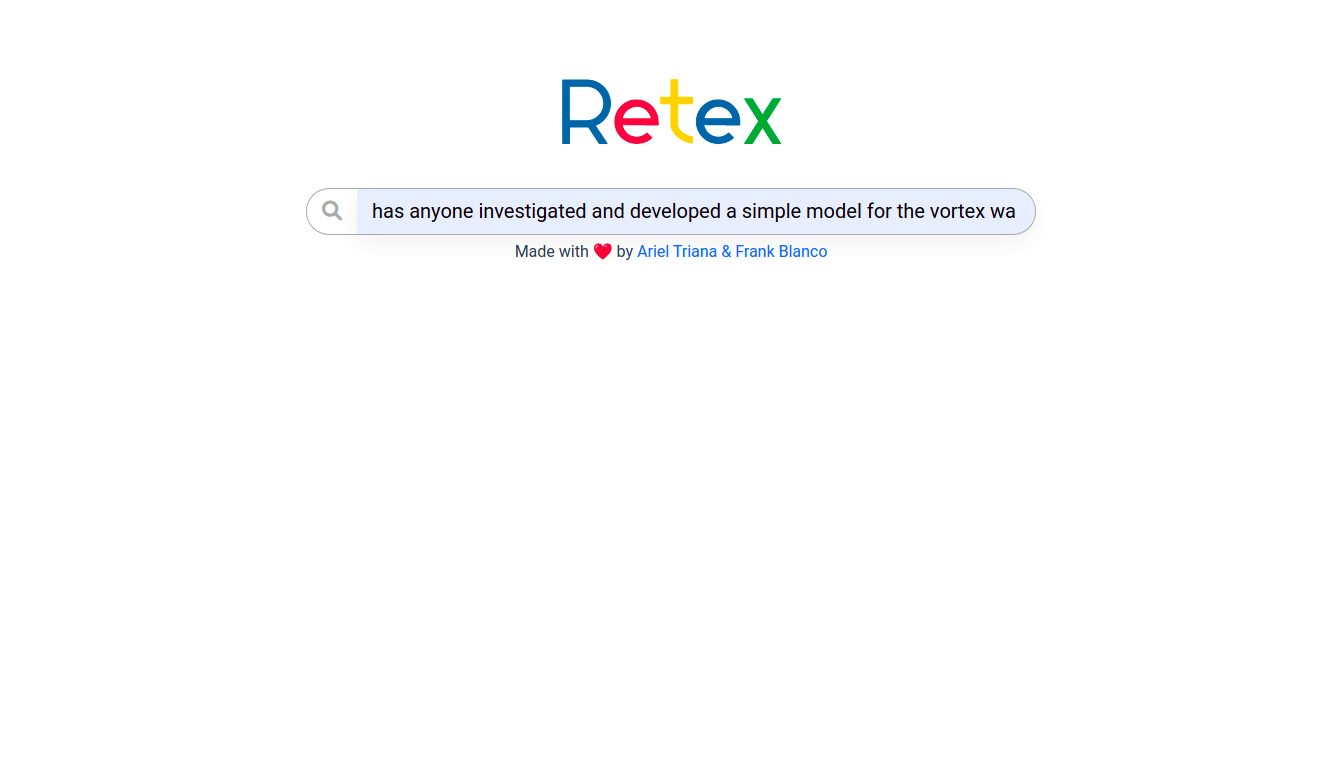
\includegraphics[width=10cm]{sections/img/home.png}
    \caption{Página de inicio de la interfaz visual con una consulta}
\end{figure}

\begin{figure}
    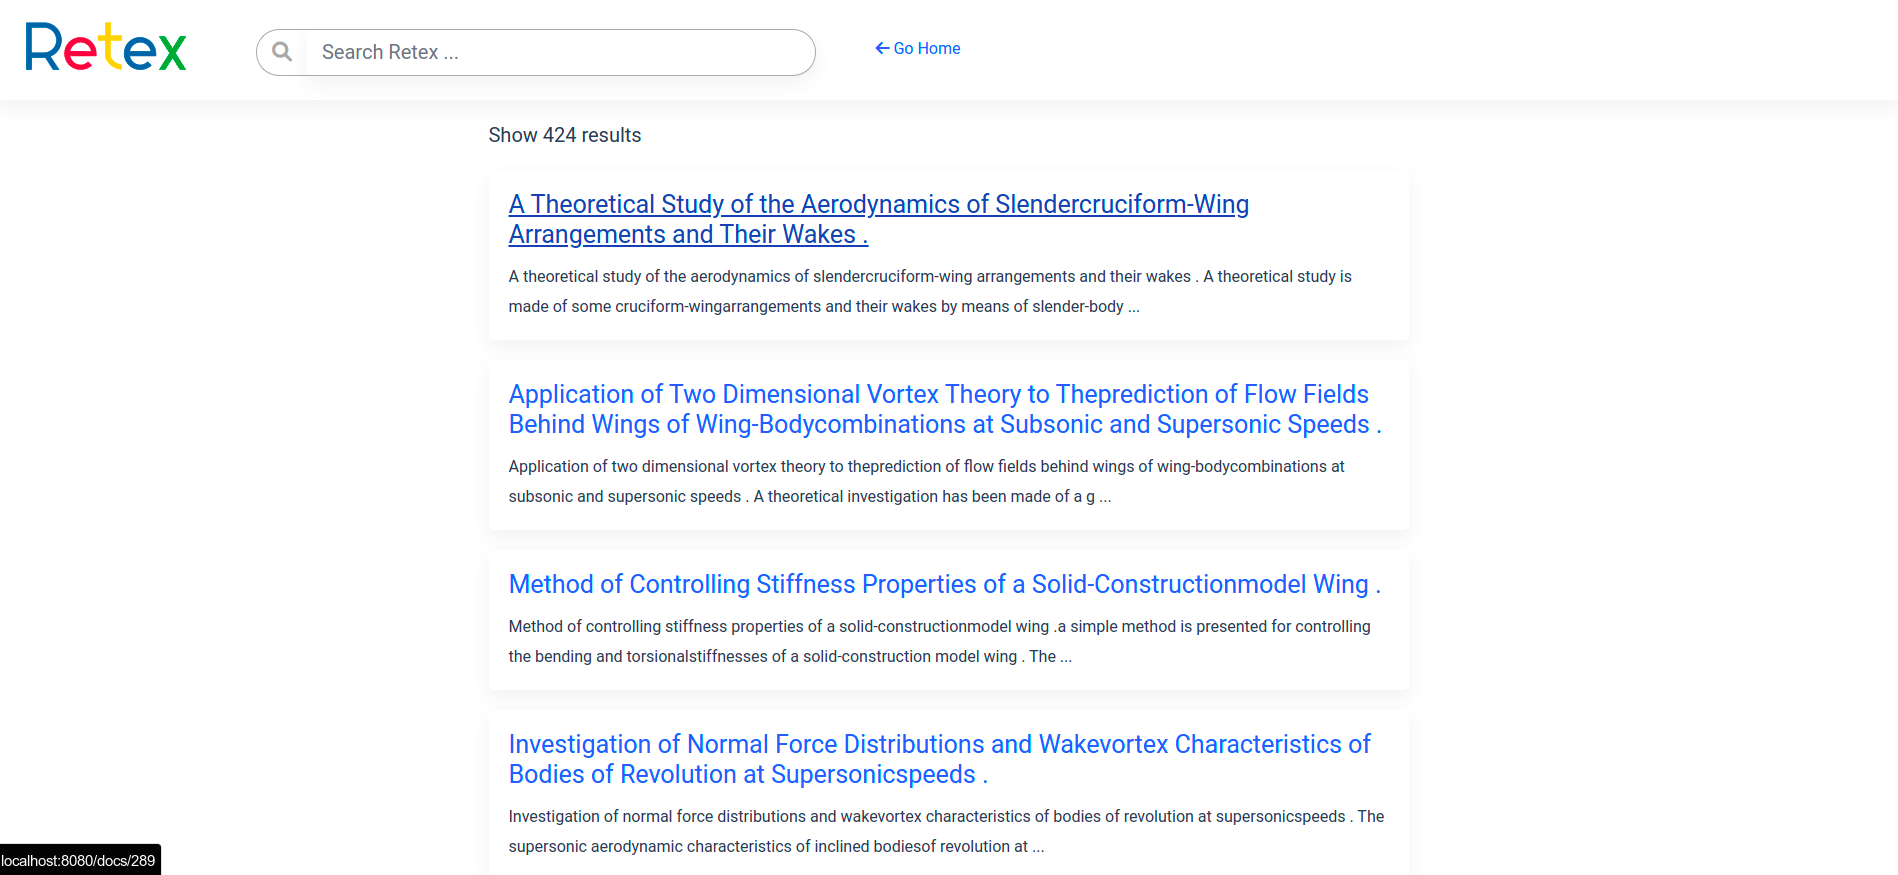
\includegraphics[width=10cm]{sections/img/result.png}
    \caption{Resultado del motor de búsqueda para la consulta realizada}
\end{figure}

\section{Ejecutando el proyecto}

El proyecto tiene 3 dependencias principales para su ejecución:

\begin{itemize}
    \item Python 3.8.10, lenguaje de programación en el cual está desarrollado todo el motor de búsqueda de Retex. 
    \item VueJS y NodeJS, framework para el desarrollo de frontends en aplicaciones web.
    \item Docker, un proyecto de código abierto que automatiza el despliegue de aplicaciones dentro de contenedores de software, proporcionando una capa adicional de abstracción y automatización de virtualización de aplicaciones en múltiples sistemas operativos.
\end{itemize}

\subsection{Instalación de dependencias}

Para instalar Docker usted debe seguir las instrucciones especificadas en la página oficial de Docker en la siguiente dirección \url{https://docs.docker.com/get-docker/}, y necesita instalar también Docker Compose siguiendo las instrucciones especificadas en la página oficial en \url{https://docs.docker.com/compose/install/}.

Una vez instalado Docker y Docker Compose, debe instalar NodeJS y el framework Vue JS, para ello siga las instrucciones en la páginas oficiales:

\begin{itemize}
    \item NodeJS: \url{https://nodejs.org/en/download/package-manager/}
    \item VueJS: \url{https://v2.vuejs.org/v2/guide/installation.html}
\end{itemize}

Debe instalar para más comodidad el software Make, siga las instrucciones aquí \url{https://www.gnu.org/software/make/}, esta dependencia es opcional.

\subsection{Ejecutando el proyecto}

Una vez instaladas todas las dependencias usted debe ejecutar en la raíz del proyecto el comando \verb|make run|, si instaló el software Make, en caso contrario ejecute el siguiente comando: \verb|docker-compose up -d --build|